\documentclass[12pt, german]{article}

\usepackage{url}
\usepackage[german]{}   % enables umlaute
\usepackage[utf8]{inputenc}  % set encoding to utf8 otherwise no umlaute
\usepackage{graphicx}        % for including graphics
\usepackage[hidelinks]{hyperref}        % for using hyperlinks in the document
\usepackage{tabularx}        % for extending tabluar
\usepackage{multirow}        % for rowspan in tabularx
\usepackage{ltablex}         % tables over multiple pages
\usepackage{textcmds}        % for quote support
\usepackage{pdfpages}        % for pdf include
\usepackage{caption}
\usepackage{minted}
\usepackage{listings}
\usepackage[left=1.0in, right=1.0in, top=1.0in, bottom=1.0in]{geometry} % for custom page layout

\newenvironment{code}{\captionsetup{type=listing}}{}

\newmintedfile[yamlFile]{yaml}{
	linenos=true, 
	frame=single, 
	breaklines=true, 
	tabsize=2,
	numbersep=5pt,
	xleftmargin=10pt,
	baselinestretch=1,
	fontsize=\footnotesize
}

\newmintedfile[javaFile]{java}{
	linenos=true, 
	frame=single, 
	breaklines=true, 
	tabsize=2,
	numbersep=5pt,
	xleftmargin=10pt,
	baselinestretch=1,
	fontsize=\footnotesize
}

\newmintedfile[groovyFile]{groovy}{
	linenos=true, 
	frame=single, 
	breaklines=true, 
	tabsize=2,
	numbersep=5pt,
	xleftmargin=10pt,
	baselinestretch=1,
	fontsize=\footnotesize
}

\newmintinline[inlineBash]{bash}{}

\usepackage{etoolbox}

\makeatletter
\AtBeginEnvironment{minted}{\dontdofcolorbox}
\def\dontdofcolorbox{\renewcommand\fcolorbox[4][]{##4}}
\makeatother

% Title Page
\title{CI/CD mit Openshift}
\author{Thomas Herzog B.Sc / Phillip Wurm B.Sc}

\setlength{\parindent}{0cm}
\sloppy
\begin{document}
\maketitle

\newpage
\tableofcontents
\newpage

\section{Problemstellung}
\label{sec:problem-statement}
hello
\section{Projektaufbau}
\label{sec:project-setup}
Dieser Abschnitt behandelt den Aufbau des Projekts \emph{CI/CD mit Openshift}. Die Quelltexte des Projekts wurden in mehreren Github \emph{Repositories} organisiert, die folgend aufgelistet sind:
\begin{enumerate}
	\item\textbf{\emph{buildserver}}\footnote{\url{https://github.com/OpenshiftCICD/buildserver}} ist das \emph{Repository}, das die Openshift \emph{Templates} und Skripten für das Aufsetzen des \emph{Build}-Servers beinhaltet.
	\item\textbf{\emph{service-jenkins}}\footnote{\url{https://github.com/OpenshiftCICD/service-jenkins}} ist das \emph{Repository}, das die Ressourcen für das Bauen des Jenkins Docker Image und der Jenkins \emph{Slave} Docker Images beinhaltet.
	\item\textbf{\emph{service-app}}\footnote{\url{https://github.com/OpenshiftCICD/service-app.git}} ist das \emph{Repository}, das die Quelltexte und die \emph{Build}-Definition der Beispielanwendung beinhaltet.
	\item\textbf{\emph{appserver}}\footnote{\url{https://github.com/OpenshiftCICD/appserver}} ist das \emph{Repository}, das die Openshift \emph{Templates} und Skripten für das Aufsetzen des Applikation Servers beinhaltet.
\end{enumerate}
\ \\
Die Aufteilung in mehrere \emph{Repositories} wurde eingeführt, da die verschiedenen \emph{Repositories} Quelltexte und Ressourcen für verschiedene Anwendungszwecke beinhalten, die nicht zwangsweise zusammenhängend sind. Z.B. beinhaltet das \emph{Repository} \emph{service-jenkins} die Ressourcen zum Bauen eines Jenkins Docker Image über einem S2I \emph{Build}, wobei das resultierende Jenkins Docker Image auch anderweitig verwendet werden kann. Daher sind die Ressourcen des \emph{Repositories service-jenkins} nicht exklusiver Teil des \emph{Build}-Servers und daher auch nicht im \emph{Repsoitory buildserver} enthalten. \\

Es werden Github \emph{Hooks} verwendet, um Openshift \emph{Builds} auszulösen, wobei bei der Aufteilung auf mehrere \emph{Repositories} Openshift \emph{Builds} nur dann ausgelöst werden, wenn die Ressourcen, die auch im \emph{Build} verwendet werden, geändert wurden. Bei der Verwendung von nur einem \emph{Repository} würden alle \emph{Builds} ausgelöst werden, was zu vielen unnötigen \emph{Builds} führen würde.
\section{Entwickler Setup}
\label{sec:dev-setup}
Dieser Abschnitt beschreibt das Aufsetzen einer lokalen Entwicklungsumgebung für die Entwicklung mit Openshift. Es wird davon ausgegangen, dass auf einem Linux System gearbeitet wird.

\subsection{Docker Setup}
Dieser Abschnitt behandelt, dass Einrichten von Docker für die Verwendung von Openshift. Es muss eine aktuelle Version von Docker installiert sein.

\begin{minted}{bash}
# 1. Define insecure registry, which is used by openshift
#    depending on your linux distribution
INSECURE_REGISTRY='--insecure-registry 172.30.0.0/16'

# 2. Reload the docker service
sudo systemctl daemon-reload

# 3.Restart the docker service
sudo systemctl restart docker
\end{minted} 

Die ungesicherte Docker \emph{Registry} wird von Openshift dazu verwendet, um in Openshift Docker Images zu verwalten. Openshift lädt sich die verwendeten externen Docker Images nur einmal in die lokale Docker \emph{Registry} und verwendet dann ausschließlich diese Images. Die in Openshift gebauten Docker Images werden ebenfalls in der lokalen Docker \emph{Registry} verwaltet.
\newpage

\subsection{Firewall Setup}
Dieser Abschnitt behandelt das Einrichten der Firewall für die Verwendung von Openshift. Ohne die folgenden Firewall Einstellungen kann in Openshift nicht auf das Internet zugegriffen werden.

\begin{minted}{bash}
# 1. Check docker bridge subnet
docker network inspect 
	-f "{{range .IPAM.Config }}{{ .Subnet }}{{end}}" bridge

# 2. Create new firewall zone
firewall-cmd --permanent --new-zone dockerc

# 3. Add docker bridge network ass source
#    The network address, is the one we got at #1
firewall-cmd --permanent --zone dockerc --add-source 172.17.0.0/16

# 4. Add all ports docker and openshift needs
firewall-cmd --permanent --zone dockerc --add-port 8443/tcp
firewall-cmd --permanent --zone dockerc --add-port 53/udp
firewall-cmd --permanent --zone dockerc --add-port 8053/udp

# 5. Reload the firewall rules
firewall-cmd --reload
	
\end{minted}


\subsection{Openshift Setup}
Dieser Abschnitt beschreibt das Einrichten des lokalen Oepnshift \emph{Clusters}. Es werden folgende Ressourcen benötigt, die aus dem Internet heruntergeladen werden können.
\begin{enumerate}
	\item\textbf{\emph{Openshift Client Tools}}\footnote{\url{https://developers.redhat.com/products/openshift/download/}} ist das Linux Paket, mit dem der lokale \emph{Cluster} erstellt werden kann.
	\item\textbf{\emph{openshift-client-wrapper}}\footnote{\url{https://github.com/openshift-evangelists/oc-cluster-wrapper/releases/tag/0.9.3}} ist ein Github \emph{Repository} das ein Shell-Skript zur Verfügung stellt, welches das Arbeiten mit oc erleichtert.
\end{enumerate}
Das \emph{oc} Binary sowie das Skript \emph{oc-cluster-wrapper} müssen in den \emph{PATH} mitaufgenommen werden. Das Skript \emph{oc-cluster-wrapper} verwendet das \emph{oc} Binary, das mit \emph{oc} über den \emph{PATH} angesprochen werden kann.
\newpage

Die folgenden \emph{Shell}-Kommandos, die von \emph{oc-cluster-wrapper} bereitgestellt werden, zeigen wie der Lebenszyklus des \emph{Clusters} gesteuert werden kann. Es wird \emph{oc-cluster-wrapper} anstatt \emph{oc} selbst verwendet, da bei \inlineBash{oc cluster down} der \emph{Cluster} vollständig gelöscht wird.
\begin{minted}{bash}
# Create or start persistent profile for local cluster named 'ci'
oc-cluster-wrapper up ci

# Stop the current running cluster (assume profile is ci)
oc-cluster-wrapper down [ci]

# Delete profile ci and all related cluster data
oc-cluster-wrapper destroy ci
\end{minted}

Wenn beim erneuten Starten eines bestehenden \emph{Cluster} Profils folgende Fehlermeldung auftritt, dann liegt es daran, dass die Konfiguration nicht mehr gültig, da der \emph{Cluster} gestartet wurde, wenn sich der Rechner in einem anderen Netz befindet als zuvor.
\begin{minted}{bash}
# Command built by oc-cluster-wrapper
oc cluster up --version v3.5.5.31 
--image registry.access.redhat.com/openshift3/ose 
--public-hostname 127.0.0.1 
--routing-suffix apps.127.0.0.1.nip.io 
--host-data-dir /home/het/.oc/profiles/ci/data 
--host-config-dir /home/het/.oc/profiles/ci/config 
--host-pv-dir /home/het/.oc/profiles/ci/pv -
-use-existing-config -e TZ=CET                                                                                                 
-- Checking OpenShift client ... OK   

...

# Resulting error, because the cluster gets startet, 
# when computer is in a different net.
Finding server IP ... 
Using 10.29.18.80 as the server IP
-- Starting OpenShift container ... FAIL
Error: Docker run error rc=2
Details:
Image: registry.access.redhat.com/openshift3/ose:v3.5.5.31
Entrypoint: [/bin/bash]
Command: [-c for name in 10.29.18.80 het.linux.gepardec.com; kma
do ls /var/lib/origin/openshift.local.config/node-$name &> /dev/null 
&& echo $name && break; done]
\end{minted}
Kopieren Sie das \emph{Shell}-Kommando \textbf{\emph{oc cluster up ...}} und entfernen Sie das Argument \textbf{\emph{--use-existing-config}}. Ohne das Argument \textbf{\emph{--use-existing-config}} wird eine neue Konfiguration erstellt.

\subsection{Ultrahook Setup}
Dieser Abschnitt behandelt das Einrichten von Ultrahook, das ein externer Service und eine lokale Applikation ist, mit der auf \emph{Localhost} auf \emph{Webhook} reagiert werden kann. Ohne Ultrahook können die \emph{Hooks} nicht lokal getestet werden. Die folgenden zwei Punkte beschreiben das Einrichten von Ultrahook.

\begin{enumerate}
	\item Registrieren eines \emph{Webhook Namespace} auf \url{http://www.ultrahook.com/register}.
	\item Starten der lokalen Anwendung mit folgenden \emph{Shell}-Kommandos\\
	\inlineBash{ultrahook -k <API_KEY> github <OPENSHIFT_HOOK_URL>}
\end{enumerate}
Jetzt kann auf einer lokalen Maschine auf z.B. Github \emph{Hooks} reagiert werden, wobei der \emph{Webhook} die von Ultrahook auf der Konsole ausgegebene \emph{Url} verwenden muss.
\section{\emph{Build Server}}
\label{sec:buildserver}
Dieser Abschnitt behandelt die Infrastruktur des \emph{Build}-Server Projekts in Openshift. 
Die Ressourcen für den \emph{Build Server} werden im \emph{Repository buildserver}\footnote{\url{https://github.com/OpenshiftCICD/buildserver}} verwaltet.

\subsection{\emph{Templates}}
\label{sec:openshift-templates}
Dieser Abschnitt behandelt die Openshift \emph{Templates}, welche die Services für die \emph{Build}-Server Infrastruktur definiert. Die Openshift \emph{Templates} beinhalten alle Definitionen wie z.B. \emph{BuildConfigurations} und \emph{Deployments}, die Aspekte des \emph{Core Conepts}\footnote{\url{https://docs.openshift.com/container-platform/3.5/architecture/core_concepts/index.html}} von Kubernetes und Openshift sind.\\

Diese Auflistung beschreibt die implementierten \emph{Templates}:
\begin{enumerate}
	\item Im \emph{Template} \textbf{\emph{jenkins-slaves.yml}} werden die für Jenkins zur Verfügung gestellten \emph{Slave-Container} verwaltet.
	\item Im \emph{Template} \textbf{\emph{jenkins.yml}} wird der Jenkins Service verwaltet.
	\item Im \emph{Template} \textbf{\emph{nexus.yml}} wird der Nexus3 Service verwaltet.
	\item Im \emph{Template} \textbf{\emph{pipeline.yml}} wird für das Anlegen einer Openshift \emph{Pipeline} verwendet.
\end{enumerate}

\ \subsection{Skripte}
Dieser Abschnitt behandelt die Skripten, die für das Verwalten des \emph{Clusters} verwendet werden. Mit der Applikation \emph{oc} kann mit dem \emph{Cluster} interagiert werden, wie z.B. PRojekte erstellen/löschen, oder Applikation in Projekten anlegen/löschen. Damit der \emph{Build Server} einfach erstellt oder gelöscht werden kann, sind für die Services und für den \emph{Build Server}   
Skripte erstellt worden, die alle nötigen Kommandos beinhalten.\\

Auf dem Level der Skripten wird eine Datei namens \emph{.openshift-env} erwartet, die Umgebungsvariablen definiert, die von Skripten verwendet wird.\\

Diese Auflistung beschreibt die implementierten \emph{Skripte}:
\begin{enumerate}
	\item Im \emph{Skript} \textbf{\emph{openshift-jenkins.sh}} sind alle Jenkins Service und Jenkins \emph{Slave} spezifischen Funktionen implementiert.
	\item Im \emph{Skript} \textbf{\emph{openshift-nexus.sh}} sind alle Jenkins Service und Jenkins \emph{Slave} spezifischen Funktionen implementiert.
	\item Im \emph{Skript} \textbf{\emph{openshift-buildserver.sh}} sind alle Funktionalitäten für das Verwalten des \emph{Build Servers} implementiert.
	\item Im \emph{Skript} \textbf{\emph{openshift-secrets.sh}} sind alle Funktionalitäten für das Verwalten von \emph{Secrets} implementiert. Siehe Abschnitt \ref{sec:buildserver-secrets} für eine genauere Beschreibung der verwendeten \emph{Secrets}.
\end{enumerate}

\ \subsection{Architektur}
Dieser Abschnitt behandelt den Aufbau des \emph{Build Servers}. Die Abbildung \ref{fig:architecture} zeigt, die Architektur des \emph{Build Server} Projekts in Openshift.
\begin{figure}[H]
	\centering
	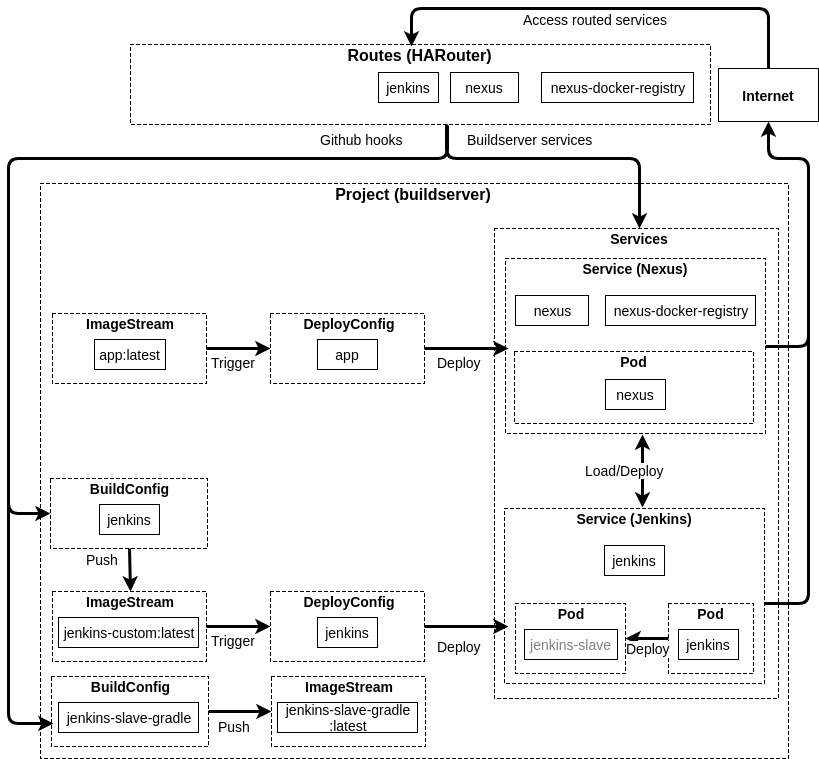
\includegraphics[scale=0.6]{logos/architecture-diagram-buildserver.jpg}
	\caption{\emph{Build Server} Architektur}
	\label{fig:architecture}
\end{figure}
\ \newpage

\section{\emph{App}-Server}
\label{sec:appserver}
Dieser Abschnitt behandelt das Openshift Projekt \emph{App}-Server, das die gebauten Services beinhaltet. In dieses Projekt wird der freigegebene Service vom Jenkins Service bzw. der Jenkins Pipeline eingespielt. Wie für den \emph{Build}-Server, beschrieben in Abschnitt \ref{sec:buildserver-scripts}, wurden auch für den \emph{App}-Server Skripte für das Verwalten des Clusters entwickelt :
\begin{enumerate}
	\item Im \emph{Skript} \textbf{\emph{openshift-appserver.sh}} sind alle Funktionalitäten für das Verwalten des \emph{App}-Servers implementiert.
	\item Im \emph{Skript} \textbf{\emph{openshift-secrets.sh}} sind alle Funktionalitäten für das Verwalten von \emph{Secrets} implementiert. Siehe Abschnitt \ref{sec:buildserver-secrets} für eine genauere Beschreibung von \emph{Secrets}.
\end{enumerate}

\begin{figure}[H]
	\centering
	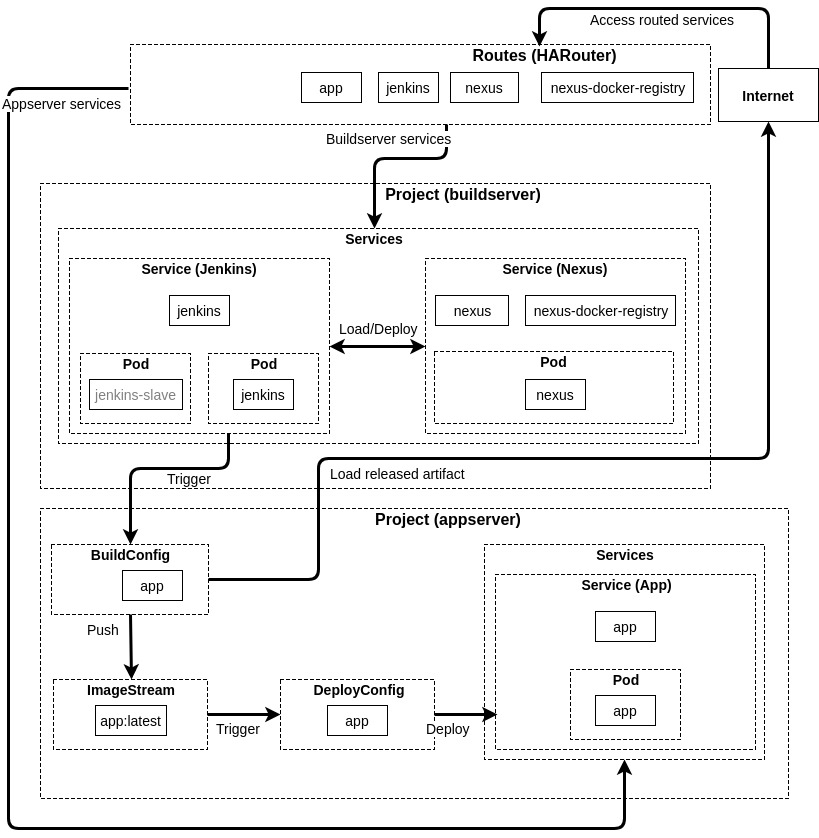
\includegraphics[scale=0.4]{logos/architecture-diagram-appserver.jpg}
	\caption{\emph{App} Server Architektur}
	\label{fig:appserver}
\end{figure}
\ \newpage

\subsection{\emph{Update}-Szenarien}
Dieser Abschnitt behandelt die \emph{Update}-Szenarien der Beispielanwendung, die in Jenkins über eine Jenkins Pipeline gebaut wird. Für diese Anwendung gibt es nur ein \emph{Update}-Szenario, nämlich wenn ein Jenkins Pipeline \emph{Build} eine neue Version freigibt, die neu eingespielt werden muss. \\

Die Jenkins Pipeline löst eine \emph{Build}-Konfiguration aus, die das neue Docker Image baut, wobei im Anschluss ein \emph{ImageChagne} Trigger ausgelöst wird, der den Service mit dem neuen Docker Image neu einspielt.
\begin{figure}[H]
	\centering
	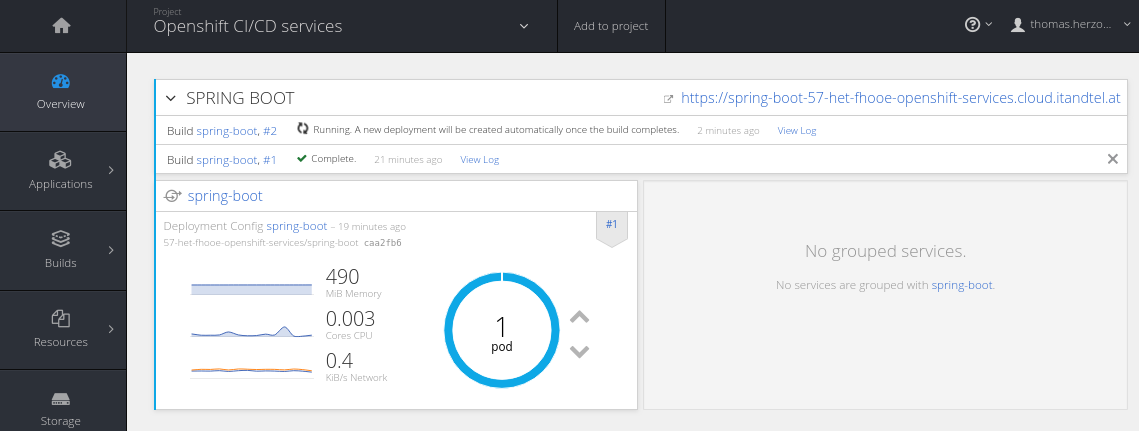
\includegraphics[scale=0.55]{image/service-app-redeploy.png}
	\caption{Ausrollen einer neuen Version des Service}
	\label{fig:appserver}
\end{figure}
\begin{figure}[H]
	\centering
	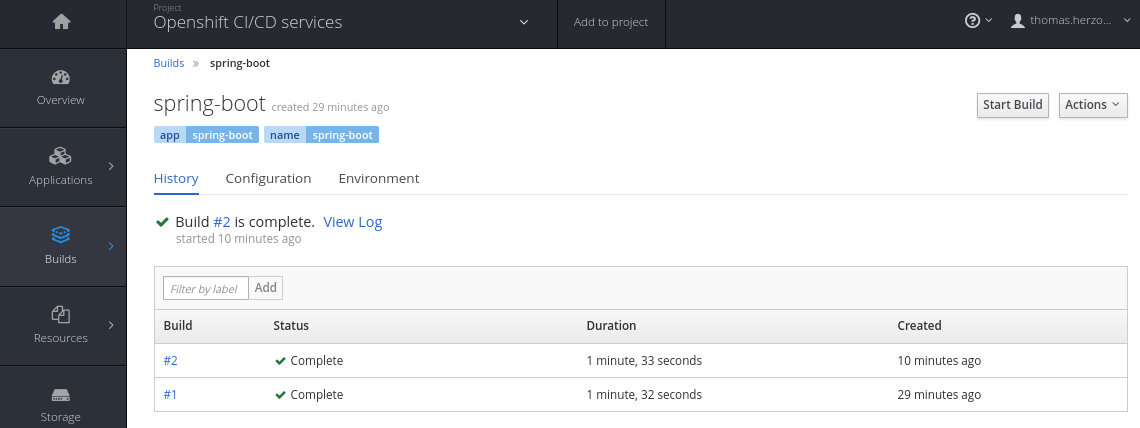
\includegraphics[scale=0.55]{image/service-app-builds.png}
	\caption{Erfolgte \emph{Builds} im \emph{App}-Server}
	\label{fig:appserver}
\end{figure}


\section{\emph{Secrets}}
\label{sec:buildserver-secrets}
Dieser Abschnitt behandelt die verwendeten \emph{Secrets}.\\

Das \emph{Secret-Objekt} oder kurz \emph{Secrets} bietet eine Möglichkt zum Speichern vertraulicher Informationen wie Passwörter, Konfigurationsdateien, dockercfg-Dateien, Anmeldeinformationen für Source-Repositorys und viele mehr. \emph{Secrets} entkoppeln sensible Inhalte von den Pods und können mithilfe eines Volumen-Plug-Ins in Containern bereitgestellt werden.

\begin{listing}[H]
	\centering
	\begin{minted}{yaml}
	apiVersion: "v1"
	kind: "Secret"
	metadata:
	  name: "test-secret"
	  namespace: "my-namespace"
	data: 
	  username: "dmFsdWUtMQ0K"
	  password: "dmFsdWUtMg0KDQo="
	stringData: 
	  hostname: "myapp.mydomain.com"
	\end{minted}
	\caption{Secret Definition}
\end{listing}

\subsection{Eigenschaften von Secrets}

Secrets können unabhängig von ihrer Definition referenziert werden. Sie werden in temporären \emph{File-storage facilities} (tmpfs) gespeichert und werden niemals auf einem Knoten abgelegt. Secrets können auch innerhalb eines Namensraums geteilt werden.

\subsection{Projekt Secrets}
\section{Jenkins \emph{Build}}
\label{sec:jenkins-build}



\subsection{Stage Prepare}

In diesem Build-Schritt werden alle Vorbereitungen für den eigentlichen Build getroffen. Es werden Variablen für \emph{Stash} und \emph{Unstash} angelegt, um das Projektverzeichnis zwischen den Steps/Pods zu verschieben. Weiters wird das aktuelle Repository verifiziert und eine Prüfsumme abgefragt.

\begin{minted}{groovy}
stage('Prepare') {
  println "Preparing the build..."
  STASH_GIT_REPO="git-repo"
  STASH_BUILD="build-result"

  println "Stashing git repo..."
  dir('../workspace@script'){
    GIT_REF = sh returnStdout: true, script: 'git rev-parse --verify HEAD'
    stash name: STASH_GIT_REPO, includes: '**/*'
  }
  println "Stashed  git repo: 'git-repo'"
  println "Prepared  the build"
}
\end{minted}

\begin{figure}[H]
	\centering
	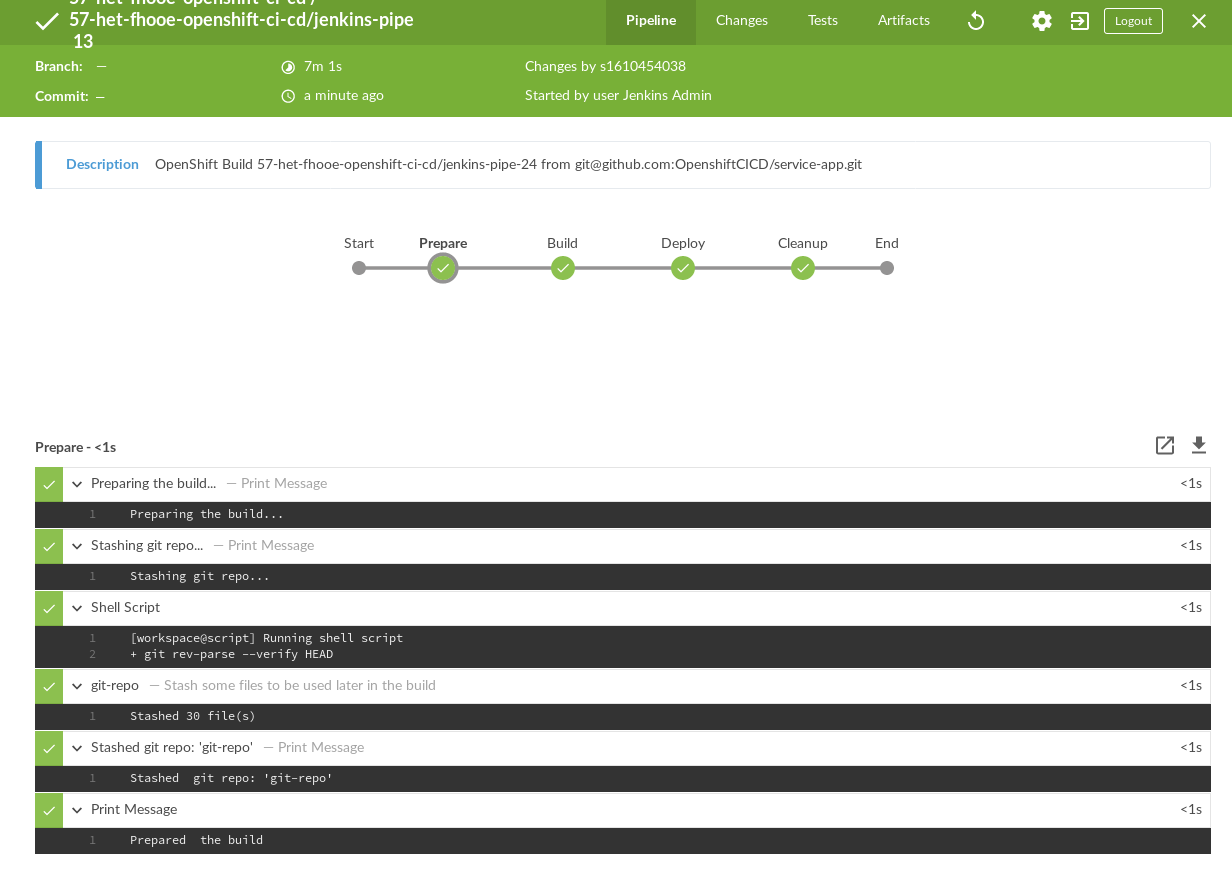
\includegraphics[scale=0.4]{image/jenkins-prepare.png}
	\caption{Prepare Build Server}
	\label{fig:architecture}
\end{figure}

\pagebreak

\subsection{Stage Build}

Der eigentliche \emph{Build} findet in einem Pod, d.h. in einem \emph{Build-Slave}, der extra dafür gestartet wird, statt. In diesem Fall wird ein \emph{Gradle-Build-Slave} gestartet, die \emph{Sourcen} werden mittels \emph{./gradle} gebaut und danach wird der \emph{Build-Slave} zerstört. Zusätzlich werden noch Umgebungsvariablen an Gradle übergeben, welche in den Build-Targets genutzt werden, um z.B. Abhängigkeiten aus einem lokalen Nexus-Repository zu laden.

\begin{minted}{groovy}
stage('Build') {
  NEXUS_USER="${env.NEXUS_USER}"
  NEXUS_PASSWORD="${env.NEXUS_PASSWORD}"
  NEXUS_MIRROR_URL="${env.MAVEN_MIRROR_URL}"
  MAVEN_REPOSITORY_URL="${env.MAVEN_REPOSITORY_URL}"

  podTemplate(name: 'jenkins-slave-gradle',
        cloud: 'openshift', containers: [
    containerTemplate(name: 'jnlp',
            image: 'ci/jenkins-slave-gradle', resourceRequestCpu: '500m', 
            resourceLimitCpu: '4000m', resourceRequestMemory: '1024Mi', 
            resourceLimitMemory: '4096Mi', slaveConnectTimeout: 180)
  ]) {
    node('jenkins-slave-gradle'){
      container('jnlp'){
        println "Unstashing '${STASH_GIT_REPO}'..."
        unstash STASH_GIT_REPO
        dir('\\complete') {
          echo sh(returnStdout: true, script: "gradle 
          -PnexusUsername=$NEXUS_USER -PnexusPassword=$NEXUS_PASSWORD 
          -PmirrorUrl=$NEXUS_MIRROR_URL 
          -PrepositoryUrl=$MAVEN_REPOSITORY_URL build")
        }
        println "Built  with gradle"
          
        println "Stashing the workspace..."
        stash name: STASH_BUILD, includes: '**/*'
        println "Stashed  the workspace"
      }
    }
  }
}
\end{minted}

\pagebreak

\subsection{Stage Deploy}

Der Trigger \emph{OpenShiftBuild} führt das Äquivalent zum Aufruf des Befehls oc start-build aus, bei dem die Build-Protokolle in Echtzeit an die Ausgabe des Jenkins-Plug-ins ausgegeben werden können. Zusätzlich zur Bestätigung, ob der Build erfolgreich war oder nicht, kann dieser Build-Schritt optional prüfen, ob die Deployment-Configs sogenannte Image-Change-Trigger für das von der Build-Config erzeugte Image haben. Wenn solche Deployment-Configs gefunden werden, werden diese  analysiert, um festzustellen, ob sie durch eine Imageänderung ausgelöst wurden. Dabei wird das vom aktuell ausgeführten Replication-Controler verwendete Image mit dem Image verglichen, das von seinem unmittelbaren Vorgänger verwendet wurde.

\begin{minted}{groovy}
stage('Deploy') {
  // Set app version on app build config
  echo sh(returnStdout: true, 
              script: "oc env buildconfigs/spring-boot VERSION=1.0.0")

  // Trigger the build config with the new version
  openshiftBuild(buildConfig: 'spring-boot', 
                       showBuildLogs: "true", 
                       checkForTriggeredDeployments: "true")
                       
   // Verify successful deployment
   openshiftVerifyDeployment(deploymentConfig: 'spring-boot', 
                                           replicaCount: "1", 
                                           verifyReplicaCount: "true",
                                            waitTime: "30000")
}
\end{minted}

\begin{figure}[H]
	\centering
	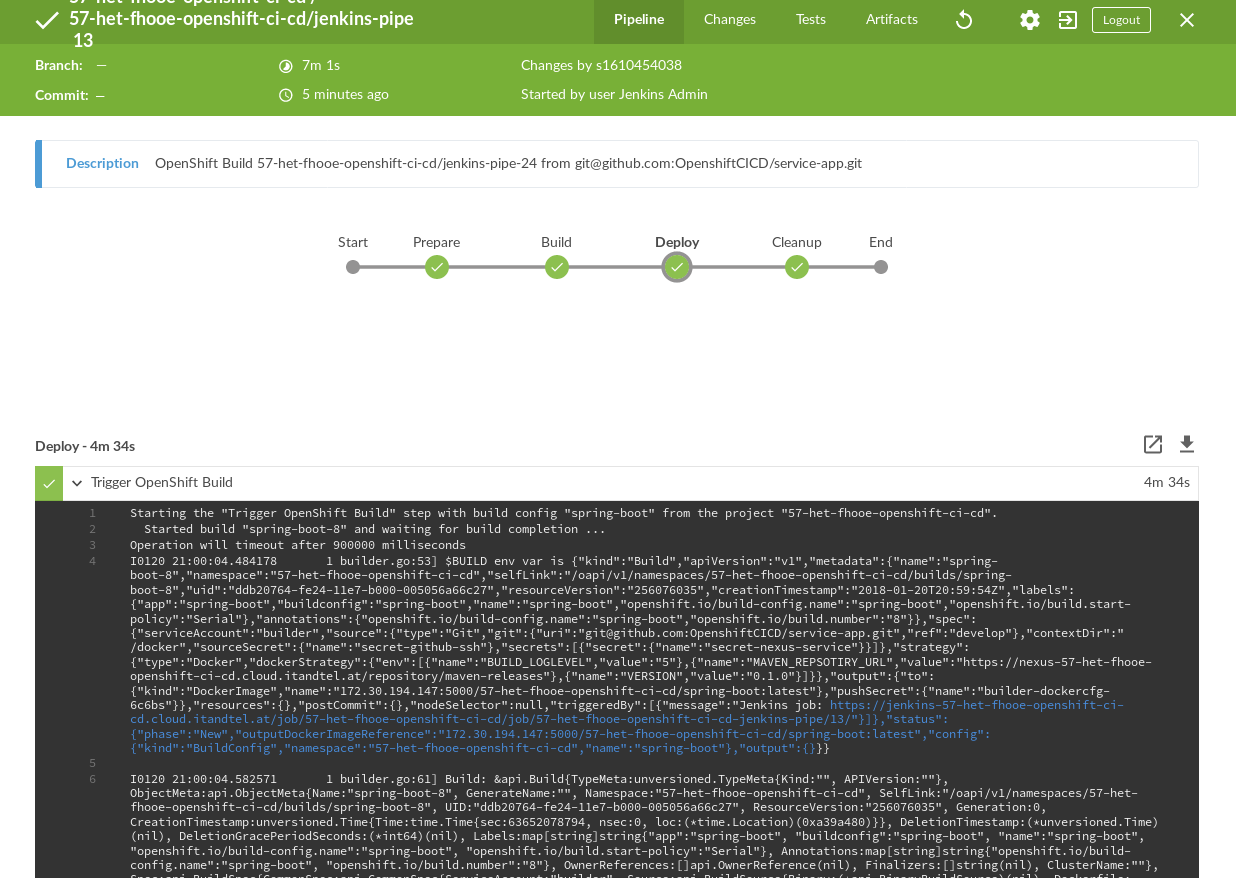
\includegraphics[scale=0.3]{image/jenkins-deploy.png}
	\caption{Deploy Build}
	\label{fig:architecture}
\end{figure}
\section{Diskussion}
\label{sec:discussion}
Dieser Abschnitt behandelt die Diskussion, des implementierten Prototypen. Die implementierte CI/CD Umgebung in Openshift war relativ einfach zu realisieren, da Jenkins und Jenkins Pipeline von Openshift nativ unterstützt werden. Da Openshift eine relativ alte Version von Jenkins und seinen Plugins zur Verfügung stellt, wurde ein eigenes Jenkins Image über einen S2I \emph{Build} definiert, das eine aktuelle Version von Jenkins und seinen Plugins zur Verfügung stellt. Das war einfach zu relaisieren und in Openshift zu integrieren, da beim Anlegen einer Jenkins Pipeline nach einem bestehenden Service mit Namen \emph{jenkins} gesucht wird, um in dieser Jenkins Instanz den Pipeline \emph{Build} anzulegen. \\

Für Jenkins und Nexus werden auch Openshift \emph{Templates} bereitgestellt, die aber angepasst wurden, um unseren Wünschen zu entsprechen. Hier verhält es sich wie bei \emph{Dockerfiles}, bei denen man auch über kurz oder lang seine eigenen \emph{Dockerfiles} implementiert anstatt die zur Verfügung gestellten zu verwenden.\\

Wenn man die Grundkonzepte, die hinter Kubernetes und Openshift stehen, verstanden hat, ist es relativ leicht mit Opensift zu arbeiten und Strukturen wie eine CI/CD Umgebung zu realisieren. Vor allem die Richtlinien wie \emph{Dockerfiles} implementiert werden sollen sind essentiell. Wenn man sich z.B. mit \inlineBash{oc rsh} in einem Docker \emph{Container} via ssh verbindet, so ist man immer ein Benutzer mit einer zufälligen \emph{uid} in der Gruppe \emph{0}, daher müssen alle Rechte so gesetzt werden, dass ein Benutzer in dieser Gruppe auch die nötigen Rechte hat. \\

Openshift verlangt auch dass immer explizit ein Benutzer in der \emph{Dockerfile} angegeben wird, mit dem der Prozess laufen soll. Standardmäßig ist es auch nicht erlaubt einen Docker Container mit \emph{Root}-Rechten zu starten. In den beiden vorherig beschriebenen Fällen wird von Openshift der Docker Container mit einer zufälligen \emph{uid} gestartet, was dazu führen kann, dass der Docker \emph{Container} nicht starten kann.


\end{document}          
